%% ============================================================================
%%  NeuroAgent / NeuroBench -- Clinical collaboration proposal deck
%%  CERN beamer theme (cafein team variant + author-year citations)
%%
%%  Build: latexmk -pdf collab_prop.tex   (or via omnilib_compile_latex)
%%  Figures live in ./figures (regenerate with: make figures)
%%  Theme + logos: ./beamerthemeCERN.sty + ./logos/
%%
%%  Audience: prospective clinical partner / hospital (validators + co-authors)
%%  Status:   scaffold only -- content to be built step by step.
%% ============================================================================

%% `table' option for xcolor must reach xcolor BEFORE beamer loads it.
\PassOptionsToPackage{table}{xcolor}

%% `t' = top-align frame bodies; matches the CERN frametitle template.
\documentclass[aspectratio=169,t]{beamer}

%% [cafein]     -> auto-wires the CAFEIN logo + appends cafein.web.cern.ch
%% [authoryear] -> citations rendered as "Protani et al. (2024)" via natbib
\usetheme[cafein,authoryear]{CERN}

%% --- Extra packages (theme already loads tikz, graphicx, booktabs, colortbl)
\usepackage{pgfplots}
\pgfplotsset{compat=1.18}
\usepackage{listings}
\usepackage{array}
\usepackage{fontawesome5}

\lstset{
  basicstyle=\ttfamily\scriptsize,
  breaklines=true,
  showstringspaces=false,
  columns=fullflexible,
  keepspaces=true,
}

\graphicspath{{figures/}{logos/}}

%% ----------------------------------------------------------------------------
%% Custom placeholder commands -- replace with real assets later.
%%  \aiplaceholder[width]{prompt-idea}   for AI-generated hero images
%%  \screenshotph[width]{caption}        for product screenshots
%% ----------------------------------------------------------------------------
\newcommand{\aiplaceholder}[2][\linewidth]{%
  \begin{tikzpicture}
    \node[draw=CERNorange, very thick, dash pattern=on 4pt off 2pt,
          rounded corners=4mm, fill=CERNorange!7,
          inner sep=2mm, align=center,
          minimum height=34mm] {%
      \parbox{\dimexpr#1-6mm\relax}{\centering
        {\bfseries\normalsize\color{CERNorange}AI HERO IMAGE}\\[0.5mm]
        {\scriptsize\itshape\color{CERNtextdark}#2}}%
    };
  \end{tikzpicture}%
}

\newcommand{\screenshotph}[2][\linewidth]{%
  \begin{tikzpicture}
    \node[draw=CERNnavy, very thick,
          rounded corners=2mm, fill=CERNlightbg,
          inner sep=2mm, align=center,
          minimum height=34mm] {%
      \parbox{\dimexpr#1-6mm\relax}{\centering
        {\bfseries\normalsize\color{CERNnavy}APP SCREENSHOT}\\[0.5mm]
        {\scriptsize\itshape\color{CERNtextdark}#2}}%
    };
  \end{tikzpicture}%
}

% Full-page screenshot placeholder (fills the entire slide, no title/footer)
\newcommand{\screenshotpage}[1]{%
  \begin{tikzpicture}[remember picture, overlay]
    \node[draw=CERNnavy, very thick, rounded corners=3mm, fill=CERNlightbg,
          inner sep=6mm, align=center,
          minimum width=\paperwidth, minimum height=\paperheight]
      at (current page.center) {%
      \parbox{0.85\paperwidth}{\centering
        {\bfseries\Large\color{CERNnavy}APP SCREENSHOT}\\[3mm]
        {\footnotesize\itshape\color{CERNtextdark}#1}}%
    };
  \end{tikzpicture}%
}

%% ----------------------------------------------------------------------------
%% Deck metadata
%% ----------------------------------------------------------------------------
\title{NeuroAgent}
\subtitle{A clinical collaboration proposal:\\
          validating an evidence-driven neurological diagnosis benchmark}
\author{Andrea Protani}
\date{\today}

\shortauthor{Andrea Protani}
\shorttitle{NeuroAgent -- collaboration proposal}
\event{Clinical collaboration proposal}

%% Pin the section list so the timeline is correct on first compile.
%% TODO: revise sections as we build the proposal narrative together.
\cernsections{Motivation, Benchmark, Validation, Agent, Results, Outlook}

\begin{document}

%% ===========================================================================
%% Cover
%% ===========================================================================
\maketitle

%% ===========================================================================
%% Motivation: Q&A is not enough -> a new paradigm
%% ===========================================================================
\begin{frame}{A new way of testing medical AI}
  \centering\footnotesize\color{CERNtextdark}
  Most research today tests medical AI with \alert{question answering}.
  Real clinical work is not like that.

  \vspace{2mm}
  \begin{columns}[T,onlytextwidth]
    \begin{column}{0.48\textwidth}
      \begin{block}{{\color{CERNblue}\faListOl}\;\, Today: question answering}
        \footnotesize
        \begin{itemize}\setlength\itemsep{0.3em}
          \item Multiple-choice exams
          \item Every clue is already in the question
          \item One correct option to pick
          \item Rewards recall, not reasoning
        \end{itemize}
      \end{block}
    \end{column}%
    \hfill
    \begin{column}{0.48\textwidth}
      \begin{alertblock}{{\color{CERNorange}\faUserInjured}\;\, Real clinical practice}
        \footnotesize
        \begin{itemize}\setlength\itemsep{0.3em}
          \item The patient arrives with a complaint, not options
          \item You decide which investigations to order
          \item Results come back over time
          \item Cost, risk and safety all matter
        \end{itemize}
      \end{alertblock}
    \end{column}
  \end{columns}

  \vspace{2mm}
  \begin{center}
  \begin{tikzpicture}
    \node[rounded corners=2mm, draw=CERNorange, line width=0.8pt,
          fill=CERNorange!10, inner sep=2.2mm,
          text width=0.9\textwidth, align=center]
    {\footnotesize\color{CERNtextdark}
      We introduce a \textbf{new paradigm}: test the AI on the
      \alert{whole diagnostic workup}, the way a clinician actually reasons.};
  \end{tikzpicture}
  \end{center}
\end{frame}

%% ===========================================================================
%% Project overview
%% ===========================================================================
\begin{frame}{Project overview}

  %% --- Step-by-step diagram: reason, test, revise -------------------------
  \begin{center}
  \begin{tikzpicture}[
    every node/.style={font=\scriptsize\sffamily, align=center},
    stage/.style={rectangle, rounded corners=2mm, very thick,
                  minimum width=20mm, minimum height=10mm,
                  align=center, inner sep=1mm},
    arr/.style={-{Stealth[length=2.2mm,width=2mm]}, very thick, CERNblue},
    larr/.style={-{Stealth[length=2.2mm,width=2mm]}, thick, dashed, CERNorange},
  ]
    \node[stage, draw=CERNnavy,   fill=CERNnavy!12]   (s1) at (0,0)
      {{\color{CERNnavy}\faUserInjured}\\\textbf{Initial}\\picture};
    \node[stage, draw=CERNblue,   fill=CERNblue!15]   (s2) at (2.9,0)
      {{\color{CERNblue}\faLightbulb}\\\textbf{Reason}\\hypothesis};
    \node[stage, draw=CERNorange, fill=CERNorange!18] (s3) at (5.8,0)
      {{\color{CERNorange}\faVial}\\\textbf{Order}\\one test};
    \node[stage, draw=CERNcyan,   fill=CERNcyan!22]   (s4) at (8.7,0)
      {{\color{CERNnavy}\faClipboardCheck}\\\textbf{Read}\\the result};
    \node[stage, draw=CERNblue,   fill=CERNblue!22]   (s5) at (11.6,0)
      {{\color{CERNblue}\faStethoscope}\\\textbf{Diagnosis}\\+ plan};

    \draw[arr] (s1) -- (s2);
    \draw[arr] (s2) -- (s3);
    \draw[arr] (s3) -- (s4);
    \draw[arr] (s4) -- (s5);
    \coordinate (lo1) at ($(s4.south)+(0,-0.34)$);
    \coordinate (lo2) at ($(s2.south)+(0,-0.34)$);
    \draw[larr, rounded corners=4pt] (s4.south) -- (lo1) -- (lo2) -- (s2.south);
    \node[font=\tiny\itshape, text=CERNorange, below=0pt]
      at ($(lo1)!0.5!(lo2)$) {revise and repeat, up to 15 steps};
  \end{tikzpicture}
  \end{center}

  \vspace{1.5mm}
  \centering\footnotesize
  \textbf{600 realistic neurology cases} across 20 conditions.

  \vspace{1.5mm}

  %% --- Two cards: what we score, why it is new -----------------------------
  \begin{columns}[T,onlytextwidth]
    \begin{column}{0.48\textwidth}
      \begin{block}{{\color{CERNblue}\faBullseye}\;\, What we measure}
        \footnotesize
        \begin{itemize}\setlength\itemsep{0.3em}
          \item Right test, right order, sensible cost
          \item Sound reasoning, not memorised facts
          \item A workup a clinician can follow
        \end{itemize}
      \end{block}
    \end{column}%
    \hfill
    \begin{column}{0.48\textwidth}
      \begin{alertblock}{{\color{CERNorange}\faLightbulb}\;\, Why it is new}
        \footnotesize
        \begin{itemize}\setlength\itemsep{0.3em}
          \item Today's AI exams hand over every clue
          \item Tests the real skill: what to investigate
          \item Each case checked by \textbf{2+ clinicians}
        \end{itemize}
      \end{alertblock}
    \end{column}
  \end{columns}
\end{frame}

%% ===========================================================================
%% The agent in action (screenshot): the goal
%% ===========================================================================
\begin{frame}{The agent in action}
  \centering\footnotesize\color{CERNtextdark}
  The goal: a transparent workup, ending in a diagnosis backed by evidence.

  \vspace{2mm}
  \tikz\node[draw=CERNnavy!35, line width=0.4pt, rounded corners=1mm,
             inner sep=0]{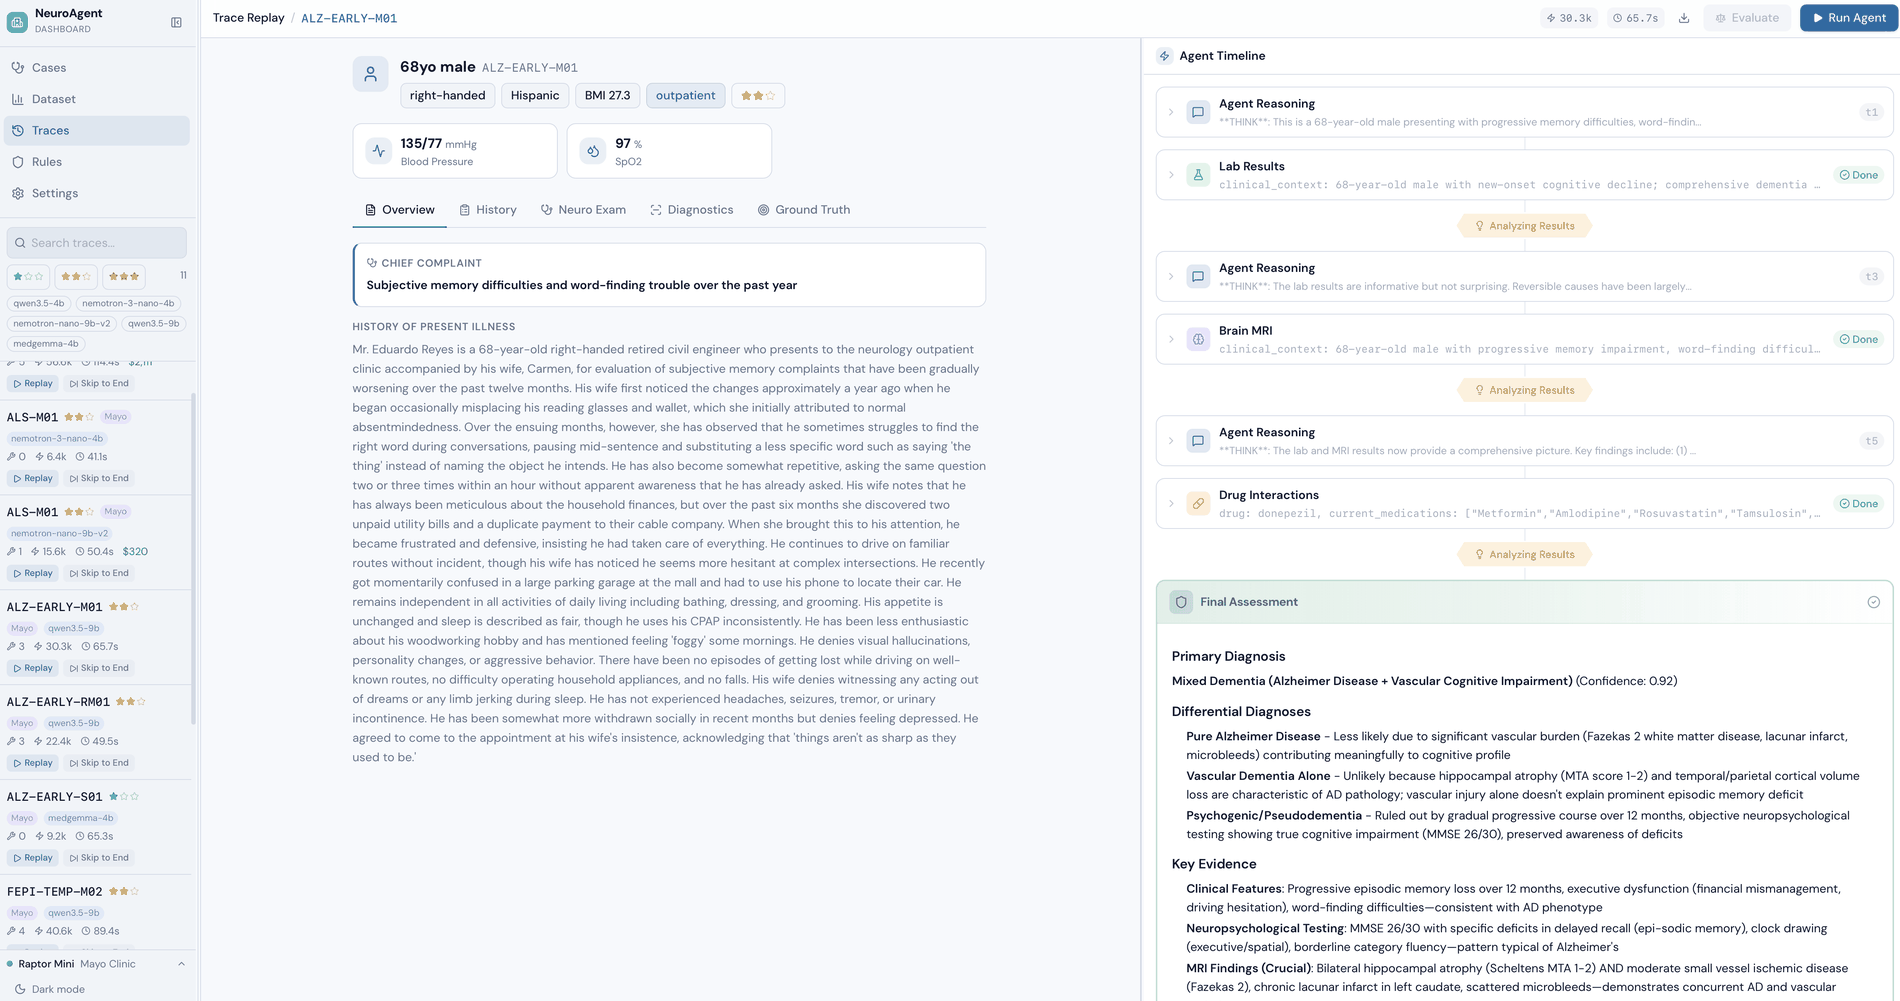
\includegraphics[height=5.5cm]{agent-in-action.png}};
\end{frame}

%% ===========================================================================
%% The dataset
%% ===========================================================================
\begin{frame}{The dataset}
  \begin{columns}[T,onlytextwidth]
    \begin{column}{0.31\textwidth}
      \begin{block}{{\color{CERNblue}\faLayerGroup}\;\, Cases}
        \centering
        \cernstatnum{600}

        \vspace{0.3mm}
        {\footnotesize 20 conditions}
      \end{block}
    \end{column}%
    \hfill
    \begin{column}{0.31\textwidth}
      \begin{alertblock}{{\color{CERNorange}\faBalanceScale}\;\, Per condition}
        \centering
        \cernstatnum[CERNorange]{30}

        \vspace{0.3mm}
        {\footnotesize exactly, fully balanced}
      \end{alertblock}
    \end{column}%
    \hfill
    \begin{column}{0.31\textwidth}
      \begin{exampleblock}{{\color{CERNcyan}\faDatabase}\;\, Follow-up results}
        \centering
        \cernstatnum[CERNcyan]{3{,}800}

        \vspace{0.3mm}
        {\footnotesize triggered by actions}
      \end{exampleblock}
    \end{column}
  \end{columns}

  \vspace{1mm}
  \begin{columns}[T,onlytextwidth]
    \begin{column}{0.48\textwidth}
      \begin{block}{{\color{CERNblue}\faSitemap}\;\, How each case is built}
        \footnotesize
        \begin{itemize}\setlength\itemsep{0.2em}
          \item Patient core: history, exam, vitals
          \item Evidence hidden behind tool calls
          \item Ground truth: best path, red herrings, unsafe actions
        \end{itemize}
      \end{block}
    \end{column}%
    \hfill
    \begin{column}{0.48\textwidth}
      \begin{alertblock}{{\color{CERNorange}\faThLarge}\;\, Spanning}
        \footnotesize
        \begin{itemize}\setlength\itemsep{0.2em}
          \item 3 difficulty tiers: straightforward to puzzle
          \item 396 synthetic + 204 real-report-seeded
          \item 3 settings: emergency / inpatient / outpatient
        \end{itemize}
      \end{alertblock}
    \end{column}
  \end{columns}

  \vspace{1mm}
  \centering\scriptsize\itshape\color{CERNtextdark}
  Results are cached in two tiers: \textbf{initial} findings when a test is
  first ordered, and \textbf{follow-ups} unlocked by a specific next action.
\end{frame}

%% ===========================================================================
%% How the cases were generated
%% ===========================================================================
\begin{frame}{How the cases were generated}
  \centering\footnotesize\color{CERNtextdark}
  Two pipelines, one schema: real cases for fidelity, synthetic cases for scale.

  \vspace{1.5mm}
  \begin{columns}[T,onlytextwidth]
    \begin{column}{0.49\textwidth}
      \begin{block}{{\color{CERNblue}\faBookMedical}\;\, Seeded from real case reports}
        \footnotesize
        \begin{itemize}\setlength\itemsep{0.25em}
          \item Source: \textbf{MedCaseReasoning}, clinician-written case reports
          \item Rewritten by \textbf{Claude Opus 4.8 + Sonnet 4.6}: findings
                hidden in tool outputs
        \end{itemize}
        \centering{\color{CERNblue}\bfseries 204 cases}
      \end{block}
    \end{column}%
    \hfill
    \begin{column}{0.49\textwidth}
      \begin{alertblock}{{\color{CERNorange}\faRobot}\;\, Fully synthetic, for scale}
        \footnotesize
        \begin{itemize}\setlength\itemsep{0.25em}
          \item Built from per-condition clinical schemas, no source report
          \item Scale needed to \textbf{fine-tune local models}
          \item Same schema and ground truth as the seeded cases
        \end{itemize}
        \centering{\color{CERNorange}\bfseries 396 cases}
      \end{alertblock}
    \end{column}
  \end{columns}

\end{frame}

%% ===========================================================================
%% The 12 tools
%% ===========================================================================
\begin{frame}{The 12 diagnostic tools}
  \scriptsize
  \begin{cerntable}{@{}p{0.30\textwidth} p{0.62\textwidth}@{}}
    \cernheaderrow
    \cernth{Tool}               & \cernth{What it returns}                              \\
    Brain MRI                   & report with region-tagged findings                   \\
    EEG                         & background, epileptiform features, focality          \\
    ECG                         & rhythm, intervals, signs of ischaemia                \\
    Labs                        & panels with reference ranges + abnormality flags     \\
    CSF (lumbar puncture)       & cells, protein, glucose, NfL, oligoclonal bands       \\
    CT scan                     & non-contrast / contrast, head / spine                \\
    Echocardiogram              & chambers, valves, ejection fraction, thrombus        \\
    Cardiac monitoring          & telemetry / Holter / loop recorder                   \\
    Advanced imaging            & MRA / MRV / CTA / PET / DaT-SPECT                    \\
    Specialised tests           & EMG/NCS, biopsy, autoimmune panels                   \\
    Literature search           & guideline and paper snippets                          \\
    Drug interactions           & interaction profile + contraindications              \\
  \end{cerntable}

  \vspace{0.5mm}
  \centering\scriptsize\itshape\color{CERNtextdark}
  Each returns a structured, typed report with a cost; any tool, any time.
\end{frame}

%% ===========================================================================
%% Mechanism: every patient is a complete picture
%% ===========================================================================
\begin{frame}{Every patient is a complete picture}
  \centering\footnotesize\color{CERNtextdark}
  Each case pre-computes a \alert{whole patient}, so the agent can order
  \textbf{any} of the 12 tools and always get a realistic answer.

  \vspace{1mm}
  \begin{center}
  \begin{tikzpicture}[
    every node/.style={font=\scriptsize\sffamily, align=center},
    box/.style={rectangle, rounded corners=2mm, very thick, inner sep=2mm,
                align=center},
    arr/.style={-{Stealth[length=2.4mm,width=2mm]}, very thick, CERNblue},
  ]
    \node[box, draw=CERNblue, fill=CERNblue!10, text width=25mm, minimum height=15mm]
      (pat) at (0,0) {{\color{CERNblue}\faUserInjured}\\\textbf{Patient}\\history, exam,\\vitals};
    \node[box, draw=CERNnavy, fill=CERNnavy!10, text width=22mm, minimum height=15mm]
      (tools) at (3.9,0) {{\color{CERNnavy}\faToolbox}\\\textbf{Any of the}\\\textbf{12 tools}};
    \node[box, draw=CERNorange, fill=CERNorange!12, text width=46mm]
      (r1) at (9.1,1.0)
      {{\color{CERNorange}\faCheckCircle}\;\textbf{On the right pathway}\\the real finding that drives the diagnosis};
    \node[box, draw=CERNcyan, fill=CERNcyan!16, text width=46mm]
      (r2) at (9.1,-1.0)
      {{\color{CERNnavy}\faMinusCircle}\;\textbf{Off pathway}\\a realistic normal or incidental result};
    \draw[arr] (pat) -- (tools);
    \draw[arr] (tools.east) -- (r1.west);
    \draw[arr] (tools.east) -- (r2.west);
  \end{tikzpicture}
  \end{center}

  \vspace{1.5mm}
  \begin{center}
  \begin{tikzpicture}
    \node[rounded corners=2mm, draw=CERNorange, line width=0.8pt, fill=CERNorange!10,
          inner sep=2.2mm, text width=0.9\textwidth, align=center]
    {\footnotesize\color{CERNtextdark}
      \textbf{Never a dead end:} every tool answers. But each call costs money
      and a turn, so ordering the wrong test is \alert{penalised}.};
  \end{tikzpicture}
  \end{center}
\end{frame}

%% ===========================================================================
%% Worked example: ISCH-STR-M02 (wake-up stroke)
%% ===========================================================================
\begin{frame}{A worked example: wake-up ischemic stroke}
  \begin{columns}[T,onlytextwidth]
    \begin{column}{0.48\textwidth}
      \begin{block}{{\color{CERNblue}\faUserInjured}\;\, Turn 1: what the agent sees}
        \footnotesize
        \begin{itemize}\setlength\itemsep{0.15em}
          \item 58\,F: woke with slurred speech, clumsy hand
          \item Last known well 9\,h ago: window unclear
          \item Left face/arm weak, sensory loss, neglect
        \end{itemize}
      \end{block}
    \end{column}%
    \hfill
    \begin{column}{0.48\textwidth}
      \begin{alertblock}{{\color{CERNorange}\faVial}\;\, What the right workup reveals}
        \footnotesize
        \begin{itemize}\setlength\itemsep{0.15em}
          \item CT first: rule out bleed; glucose: no hypoglycemia
          \item MRI: fresh infarct, deep right white matter
          \item ECG, echo, carotids, Holter: hunt the cause
        \end{itemize}
      \end{alertblock}
    \end{column}
  \end{columns}

  \vspace{1mm}
  \begin{exampleblock}{{\color{CERNcyan}\faMinusCircle}\;\, The trap, and an off-pathway test}
    \footnotesize
    \alert{``Chronic, not acute''} tempts an early stop, yet the cause hunt is still owed. An off-pathway EEG reads \textbf{normal}: wasted.
  \end{exampleblock}

  \vspace{0.5mm}
  \centering\footnotesize\color{CERNnavy}
  {\faNotesMedical}\;\textbf{Ground truth:} acute ischemic stroke, right corona radiata (ICD-10 I63.541).
\end{frame}

%% ===========================================================================
%% How we evaluate performance
%% ===========================================================================
\begin{frame}{How we evaluate performance}
  \vspace{1mm}
  \begin{columns}[T,onlytextwidth]
    \begin{column}{0.49\textwidth}
      \begin{block}{{\color{CERNblue}\faCalculator}\;\, Automatic metrics, per case}
        \footnotesize
        \begin{itemize}\setlength\itemsep{0.15em}
          \item \textbf{Diagnosis:} ICD top-1 / top-3 match
          \item \textbf{Tool selection:} precision, recall, F1 + coverage
          \item \textbf{Safety:} contraindicated, harmful, wrong-order calls
          \item \textbf{Cost:} \$ vs optimal; useless or repeated calls
        \end{itemize}
      \end{block}
    \end{column}%
    \hfill
    \begin{column}{0.49\textwidth}
      \begin{alertblock}{{\color{CERNorange}\faGavel}\;\, AI reasoning judge, 0--5 each}
        \footnotesize
        \begin{itemize}\setlength\itemsep{0.15em}
          \item Diagnostic accuracy; evidence found + integrated
          \item Differential reasoning; uncertainty calibration
          \item Tool efficiency, safety, red-herring handling
          \item One \textbf{composite reasoning score}
        \end{itemize}
      \end{alertblock}
    \end{column}
  \end{columns}

  \vspace{1mm}
  \begin{exampleblock}{{\color{CERNcyan}\faUserMd}\;\, Clinician validation: the gold standard}
    \footnotesize
    $\geq$2 clinicians per case: field-level approval + inter-rater agreement, the human ceiling we calibrate against.
  \end{exampleblock}
\end{frame}

%% ===========================================================================
%% What we are asking: the collaboration
%% ===========================================================================
\begin{frame}{What we are asking of you}
  \centering\footnotesize\color{CERNtextdark}
  \begin{columns}[T,onlytextwidth]
    \begin{column}{0.49\textwidth}
      \begin{block}{{\color{CERNblue}\faStethoscope}\;\, 1.\ Validate the cases}
        \footnotesize
        \begin{itemize}\setlength\itemsep{0.2em}
          \item Read each patient as you would in clinic
          \item Approve, flag, or correct field by field
          \item Drop cases that are not good enough
        \end{itemize}
      \end{block}
    \end{column}%
    \hfill
    \begin{column}{0.49\textwidth}
      \begin{alertblock}{{\color{CERNorange}\faGavel}\;\, 2.\ Validate our scoring}
        \footnotesize
        \begin{itemize}\setlength\itemsep{0.2em}
          \item Score a sample of agent runs yourself
          \item Compare against the AI reasoning judge
          \item Confirm scores track clinical quality
        \end{itemize}
      \end{alertblock}
    \end{column}
  \end{columns}

  \vspace{1.5mm}
  \begin{exampleblock}{{\color{CERNcyan}\faUsers}\;\, How the review works}
    \footnotesize
    \begin{itemize}\setlength\itemsep{0.15em}
      \item $\geq$\textbf{2 independent reviewers} per case
      \item Separate login per reviewer: blind, no shared bias
      \item Agreement stats $\rightarrow$ fix or drop weak cases $\rightarrow$ higher quality
    \end{itemize}
  \end{exampleblock}
\end{frame}

%% ===========================================================================
%% The annotation platform (screenshots): browse + case view
%% ===========================================================================
\begin{frame}{The annotation platform}
  \begin{columns}[T,onlytextwidth]
    \begin{column}{0.49\textwidth}
      \centering
      \tikz\node[draw=CERNnavy!35, line width=0.4pt, rounded corners=1mm,
                 inner sep=0]{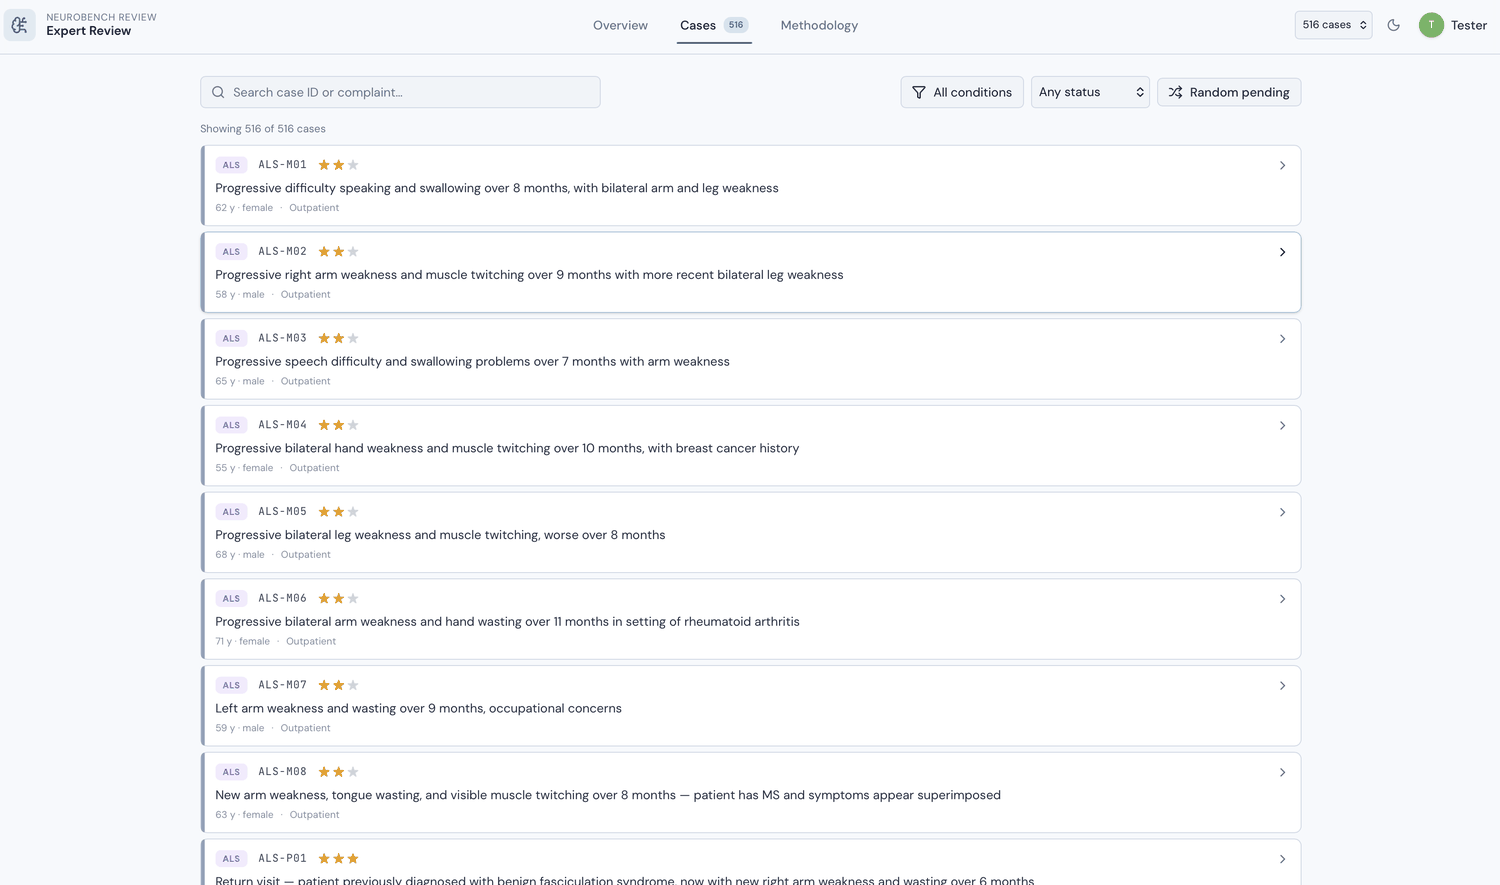
\includegraphics[height=4.0cm]{review-cases.png}};

      \vspace{0.8mm}
      {\scriptsize\color{CERNnavy}\faThList\;\, Browse cases: condition, difficulty, status}
    \end{column}%
    \hfill
    \begin{column}{0.49\textwidth}
      \centering
      \tikz\node[draw=CERNnavy!35, line width=0.4pt, rounded corners=1mm,
                 inner sep=0]{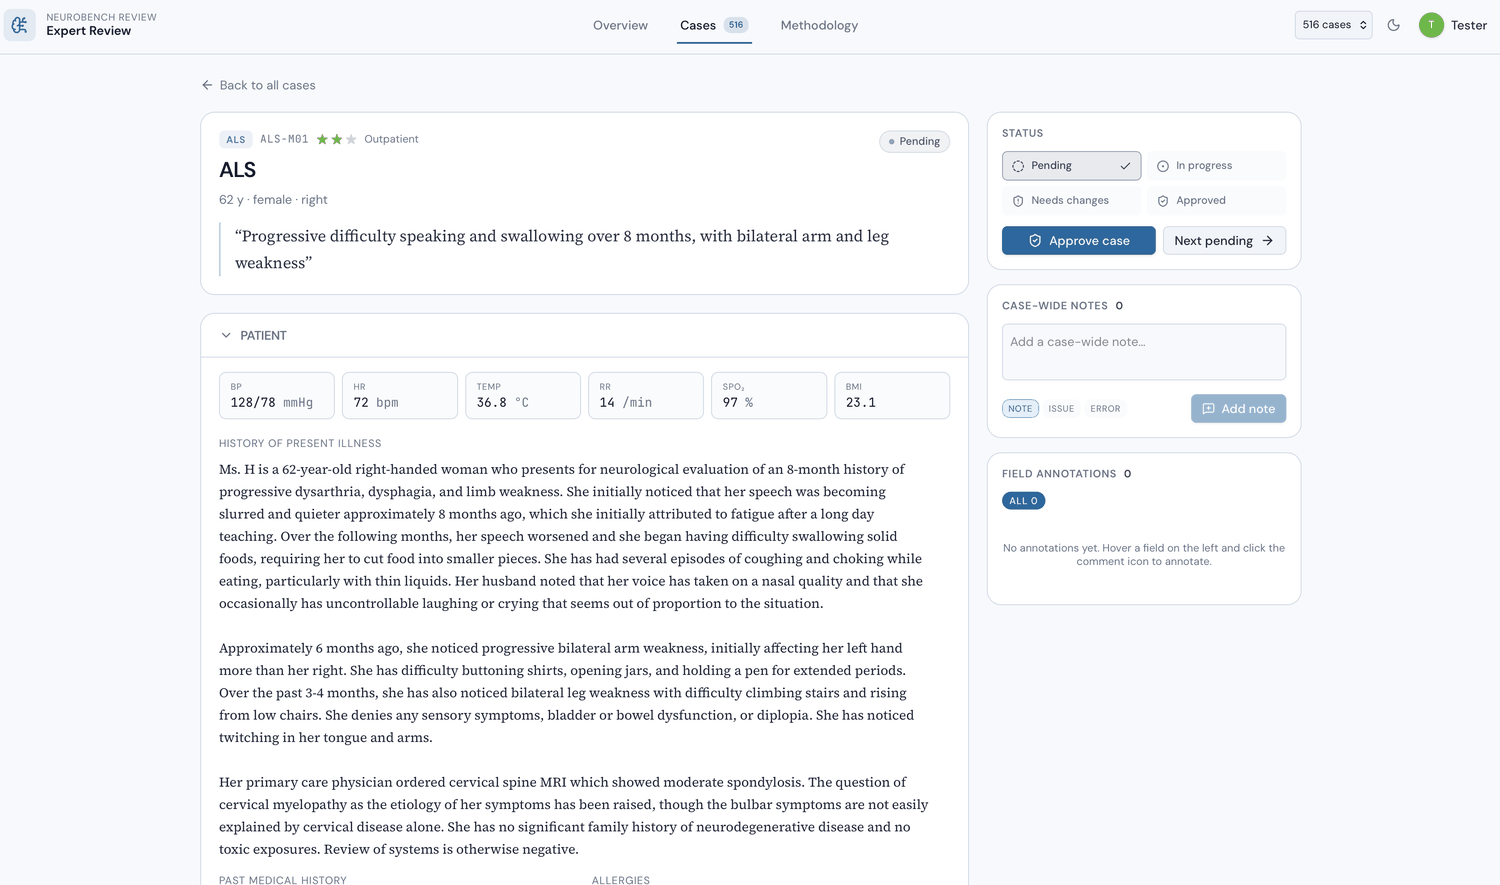
\includegraphics[height=4.0cm]{review-case.png}};

      \vspace{0.8mm}
      {\scriptsize\color{CERNnavy}\faUserInjured\;\, One screen per patient: vitals, history, full workup}
    \end{column}
  \end{columns}

\end{frame}

%% ===========================================================================
%% Reviewing a case: annotate + status
%% ===========================================================================
\begin{frame}{Reviewing a case}
  \begin{columns}[T,onlytextwidth]
    \begin{column}{0.62\textwidth}
      \centering
      \tikz\node[draw=CERNnavy!35, line width=0.4pt, rounded corners=1mm,
                 inner sep=0]{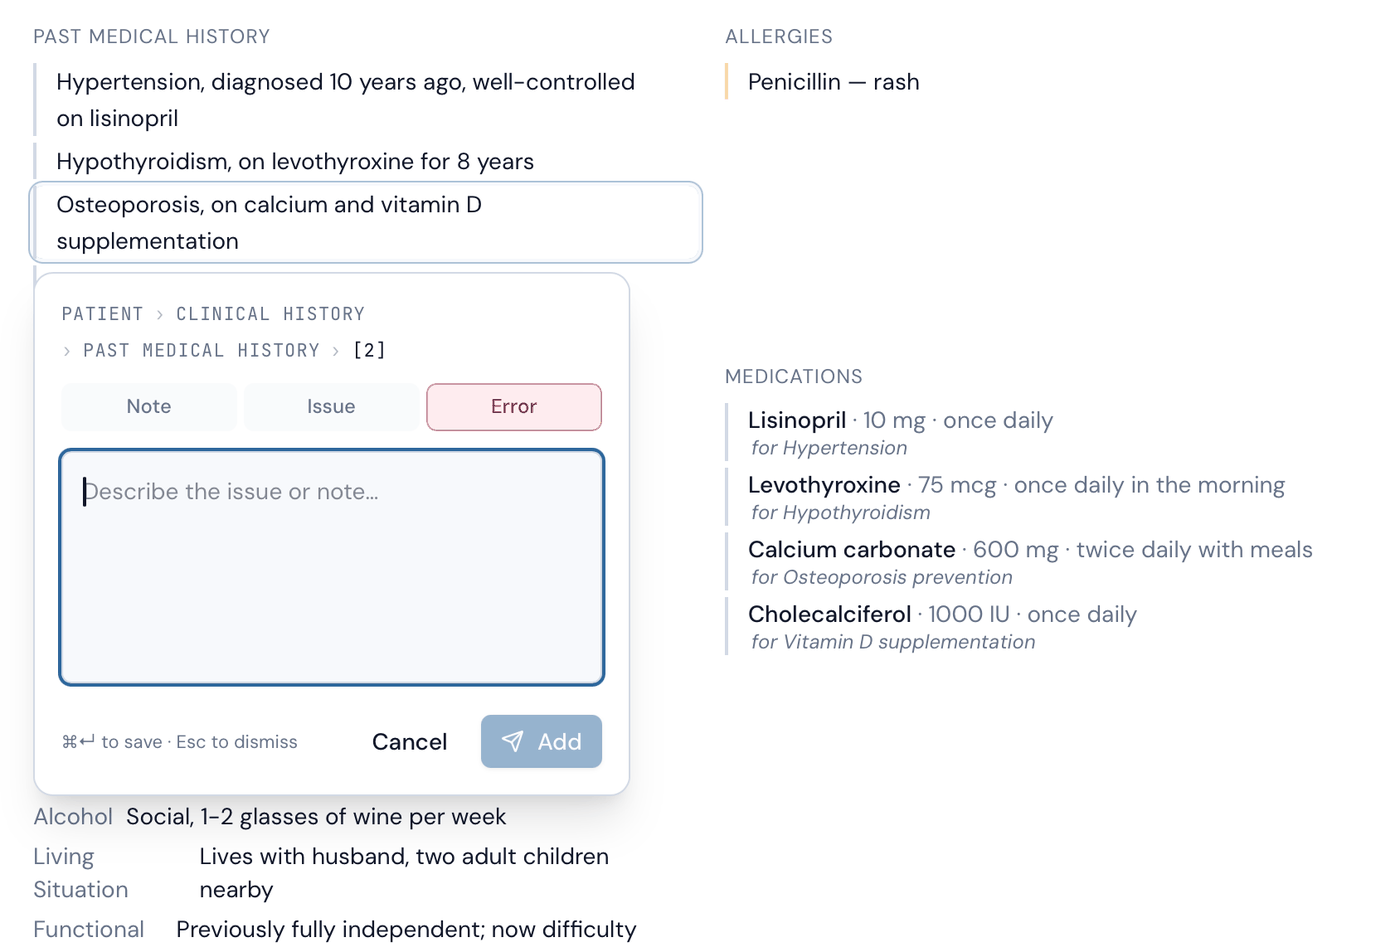
\includegraphics[height=4.3cm]{review-annotate.png}};

      \vspace{1.2mm}
      {\scriptsize\color{CERNnavy}\faCommentDots\;\, Flag any field: note, issue, or error}
    \end{column}%
    \hfill
    \begin{column}{0.36\textwidth}
      \centering
      \tikz\node[draw=CERNnavy!35, line width=0.4pt, rounded corners=1mm,
                 inner sep=0]{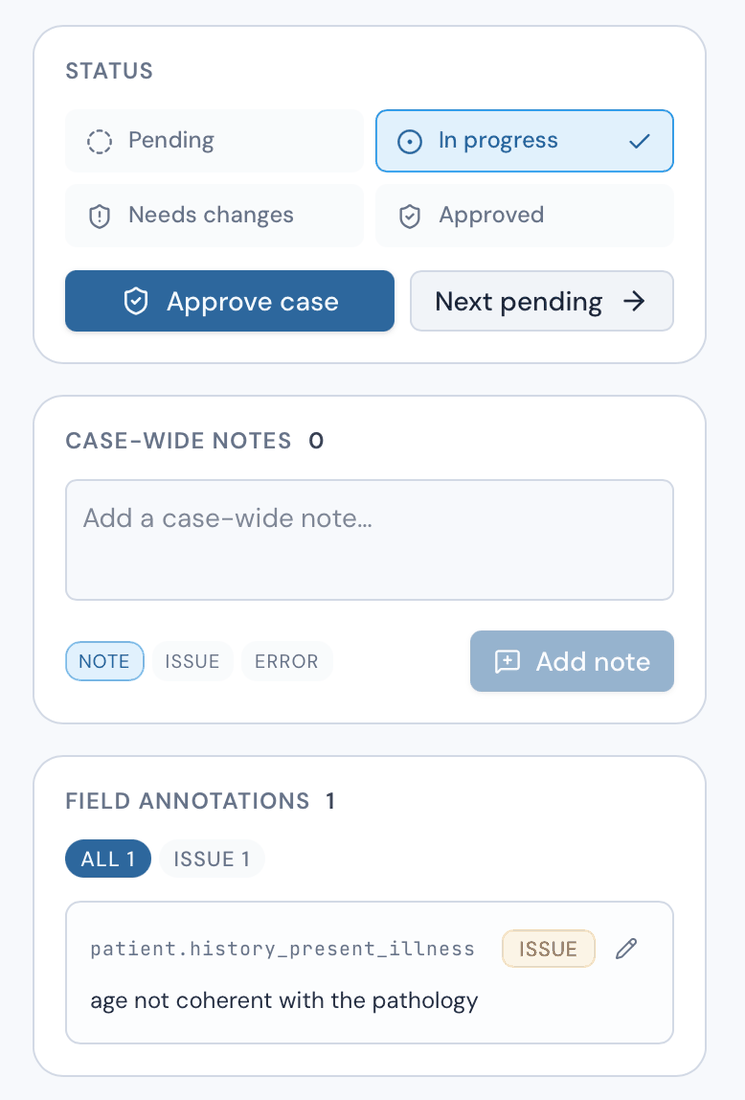
\includegraphics[height=4.3cm]{review-status.png}};

      \vspace{1.2mm}
      {\scriptsize\color{CERNnavy}\faTasks\;\, Per-case status, every annotation logged}
    \end{column}
  \end{columns}

  \vspace{2mm}
  \centering\scriptsize\itshape\color{CERNtextdark}
  Approve, request changes, or move on: progress tracked per reviewer.
\end{frame}

%% ===========================================================================
%% End slide
%% ===========================================================================
\makeend

\end{document}
